% L10c bandit figure: four arms, each with a reward distribution on [0, 1] that
% the agent cannot see, and one pulled arm that reports a single reward.
%
% Drawn on October 20, 2026 with the palette and build of the L10a figures.
%
% Each arm is a vertical reward axis (0 at the bottom, 1 at the top, 4 cm per
% unit reward) with its reward density drawn to the right of the axis
% (0.5 cm per unit density). The densities are Beta distributions, the family
% the lab's arms use; the parameters, normalizing constants 1/B(a, b), and
% means are:
%   arm 1: Beta(3, 5), 105, mean 3/8 = 0.375
%   arm 2: Beta(5, 4), 280, mean 5/9 = 0.556  (the pulled arm)
%   arm 3: Beta(7, 3), 252, mean 7/10 = 0.700 (the best arm, mu star)
%   arm 4: Beta(4, 5), 280, mean 4/9 = 0.444
% The pulled arm reports one draw, r_t = 0.45. The dashed line is mu star, and
% the red bracket is the gap Delta(1) = 0.700 - 0.375 = 0.325.
%
% Labels are set large so they stay readable when the slide scales the figure
% down (October 22, 2026). Math uses the standard TeX fonts (no unicode-math),
% so symbols render as the notebook's math shows them.
%
% The notebook SVG carries a dark palette added by theme_svg.py; keep new
% colors in that script's mapping when changing the palette here.
\documentclass[tikz,border=4pt]{standalone}
\usepackage[no-math]{fontspec}
\IfFontExistsTF{Arial}{\setsansfont{Arial}}{\setsansfont{TeX Gyre Heros}}
\renewcommand{\familydefault}{\sfdefault}
\usepackage{amsmath,amssymb}

% Ink, blue, red, gray, and band match the L10a figures. Red marks the gap,
% how much less arm 1 earns on average than the best arm.
\definecolor{vnink}{HTML}{202124}
\definecolor{gdblue}{HTML}{0091FF}
\definecolor{gdred}{HTML}{E02020}
\definecolor{gdgray}{HTML}{6D7278}
\definecolor{waband}{HTML}{EEF0F2}
\definecolor{bafill}{HTML}{B3DCFF}

% \density{axis x}{alpha}{beta}{1/B(alpha, beta)}{fill}{edge}: a Beta density
% drawn to the right of a vertical reward axis.
\newcommand{\density}[6]{%
  \filldraw[fill=#5, draw=#6, line width=0.8pt]
    plot[domain=0:1, samples=201]
      ({#1 + 0.5*#4*(\x)^(#2 - 1)*(1 - \x)^(#3 - 1)}, {4*\x}) -- cycle;}
% \meantick{axis x}{alpha}{beta}{1/B(alpha, beta)}{mean}: the mean reward, a
% tick from the axis to the edge of the density.
\newcommand{\meantick}[5]{%
  \pgfmathsetmacro{\w}{0.5*#4*(#5)^(#2 - 1)*(1 - #5)^(#3 - 1)}
  \draw[vnink, line width=1.2pt] (#1, 4*#5) -- (#1 + \w, 4*#5);}

\begin{document}
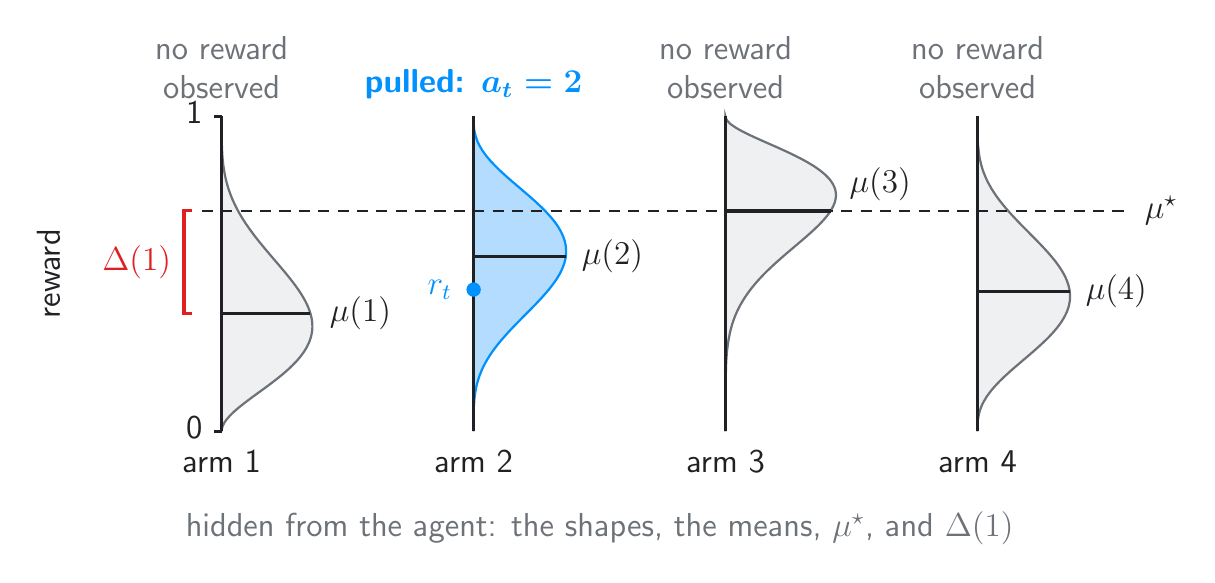
\begin{tikzpicture}[x=1cm, y=1cm, font=\sffamily\large, text=vnink,
    cell/.style={text height=1.6ex, text depth=0.45ex},
  ]
  % reward densities, the pulled arm in blue
  \density{0}{3}{5}{105}{waband}{gdgray}
  \density{3.2}{5}{4}{280}{bafill}{gdblue}
  \density{6.4}{7}{3}{252}{waband}{gdgray}
  \density{9.6}{4}{5}{280}{waband}{gdgray}

  % the best mean reward, mu star
  \draw[vnink, line width=0.8pt, dash pattern=on 4pt off 3pt] (-0.25, 2.8) -- (11.55, 2.8);
  \node[anchor=west] at (11.6, 2.8) {$\mu^\star$};

  % mean reward ticks and labels
  \meantick{0}{3}{5}{105}{0.375}
  \meantick{3.2}{5}{4}{280}{0.5556}
  \meantick{6.4}{7}{3}{252}{0.7}
  \meantick{9.6}{4}{5}{280}{0.4444}
  \node[anchor=west] at (1.25, 1.5) {$\mu(1)$};
  \node[anchor=west] at (4.45, 2.222) {$\mu(2)$};
  \node[anchor=south west] at (7.85, 2.8) {$\mu(3)$};
  \node[anchor=west] at (10.85, 1.778) {$\mu(4)$};

  % reward axes, with the reward scale on the first one
  \foreach \x in {0, 3.2, 6.4, 9.6} \draw[vnink, line width=0.9pt] (\x, 0) -- (\x, 4);
  \foreach \y/\v in {0/0, 4/1} {
    \draw[vnink, line width=0.9pt] (-0.1, \y) -- (0, \y);
    \node[cell, anchor=east] at (-0.12, \y) {\v};
  }
  \node[rotate=90] at (-2.2, 2) {reward};

  % the gap of arm 1
  \draw[gdred, line width=1.2pt] (-0.38, 1.5) -- (-0.48, 1.5) -- (-0.48, 2.8) -- (-0.38, 2.8);
  \node[anchor=east, text=gdred] at (-0.52, 2.15) {$\Delta(1)$};

  % the pulled arm and its one observed reward
  \fill[gdblue] (3.2, 1.8) circle (2.6pt);
  \node[anchor=east, text=gdblue] at (3.05, 1.8) {$r_t$};
  \node[anchor=south, text=gdblue, font=\sffamily\large\bfseries] at (3.2, 4.1) {pulled: $\boldsymbol{a_t=2}$};
  \foreach \x in {0, 6.4, 9.6} \node[anchor=south, text=gdgray, align=center] at (\x, 4.1) {no reward\\observed};

  % arm names
  \foreach \i/\x in {1/0, 2/3.2, 3/6.4, 4/9.6} \node[cell, anchor=north] at (\x, -0.15) {arm \i};

  % what we drew but the agent cannot see
  \node[anchor=north, text=gdgray] at (4.8, -0.9) {hidden from the agent: the shapes, the means, $\mu^\star$, and $\Delta(1)$};
\end{tikzpicture}
\end{document}
